\documentclass[10pt]{beamer}
\usepackage{ctex}
\setCJKmainfont{宋体}

\usetheme{metropolis}
\usepackage{appendixnumberbeamer}

\usepackage{booktabs}
\usepackage[scale=2]{ccicons}

\usepackage{pgfplots}
\usepgfplotslibrary{dateplot}

\usepackage{xspace}
\newcommand{\themename}{\textbf{\textsc{metropolis}}\xspace}

\title{基于深度学习的求解图像逆问题的方法研究}
\subtitle{毕设答辩}
\date{\today}
\author{张珏烨}
\institute{武汉理工大学计算机与人工智能学院}
% \titlegraphic{\hfill\includegraphics[height=1.5cm]{logo.pdf}}

\begin{document}

\maketitle

\begin{frame}{目录}
  \setbeamertemplate{section in toc}[sections numbered]
  \tableofcontents[hideallsubsections]
\end{frame}

\section{引言}

\begin{frame}[fragile]{AI带来的恐惧}
  \begin{figure}[thbp!]
    \centering
    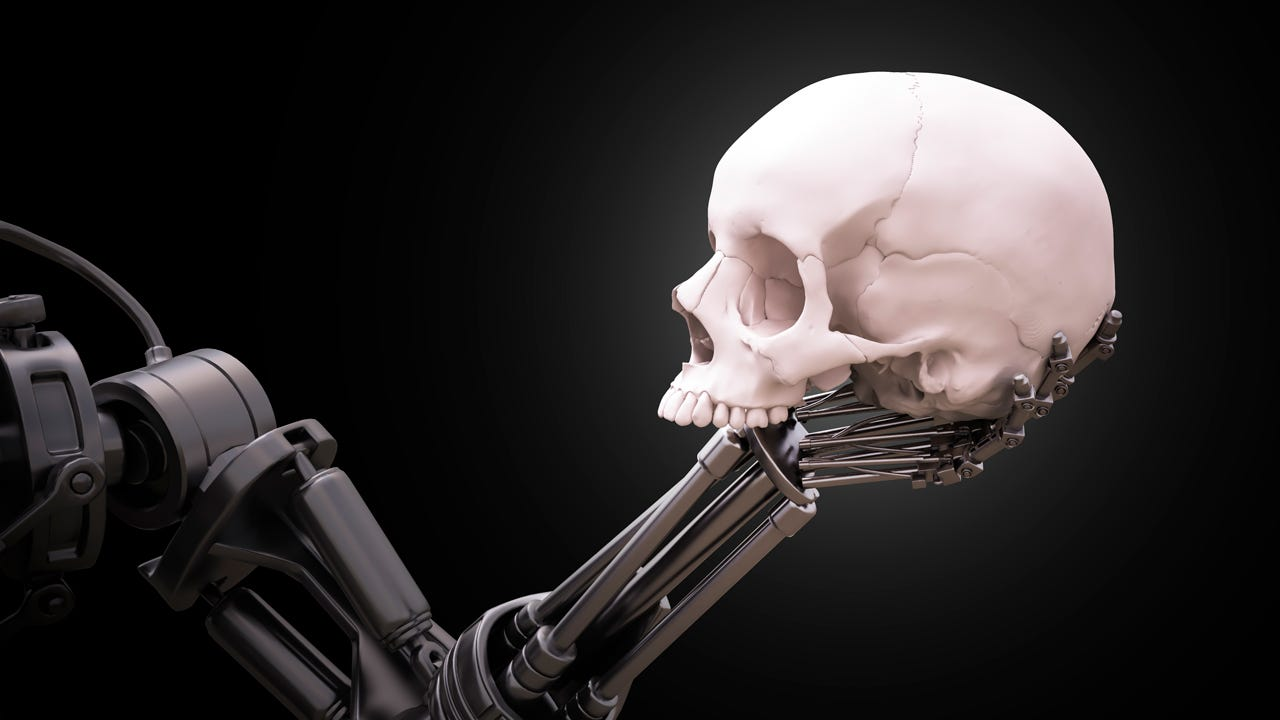
\includegraphics[width=0.8\linewidth]{imgs/ai.jpg}
    \caption{Evil AI}
    \label{fig:evil-ai}
    \end{figure}
  \begin{itemize}
    \item 随着GPT的爆火,人们越来越恐惧于AI强大的学习和推理能力
    \item 如何提升AI的可解释性,加强人们对AI的理解和控制,迫在眉睫
  \end{itemize}
\end{frame}

\begin{frame}[fragile]{神经科学}
  \begin{figure}[thbp!]
    \centering
    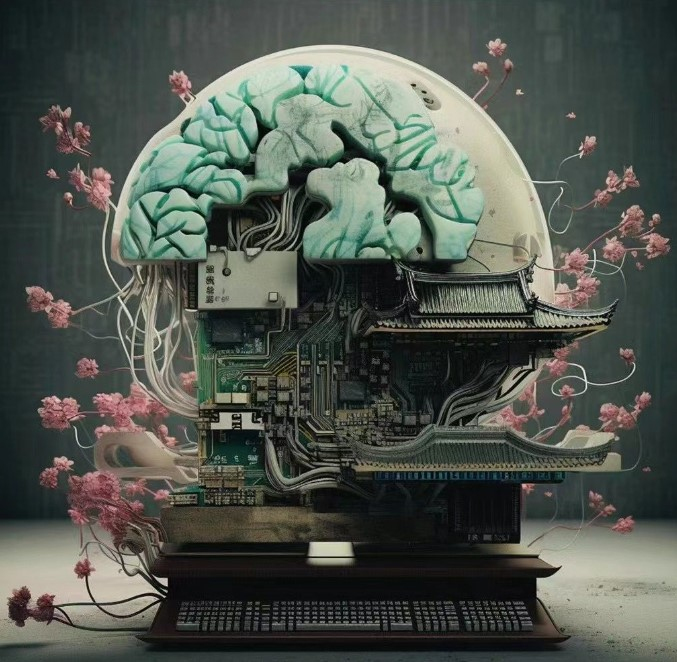
\includegraphics[width=0.5\linewidth]{imgs/CCN.jpg}
    \caption{NeuroAI}
    \label{fig:NeuroAI}
    \end{figure}
  
  \begin{itemize}
    \item 神经科学作为神经网络的起源,可能是可解释性AI的一条通路
    \item 不过,人类对神经科学同样知之甚少
  \end{itemize}
\end{frame}

\begin{frame}[fragile]{连接组学}
  \begin{figure}[thbp!]
    \centering
    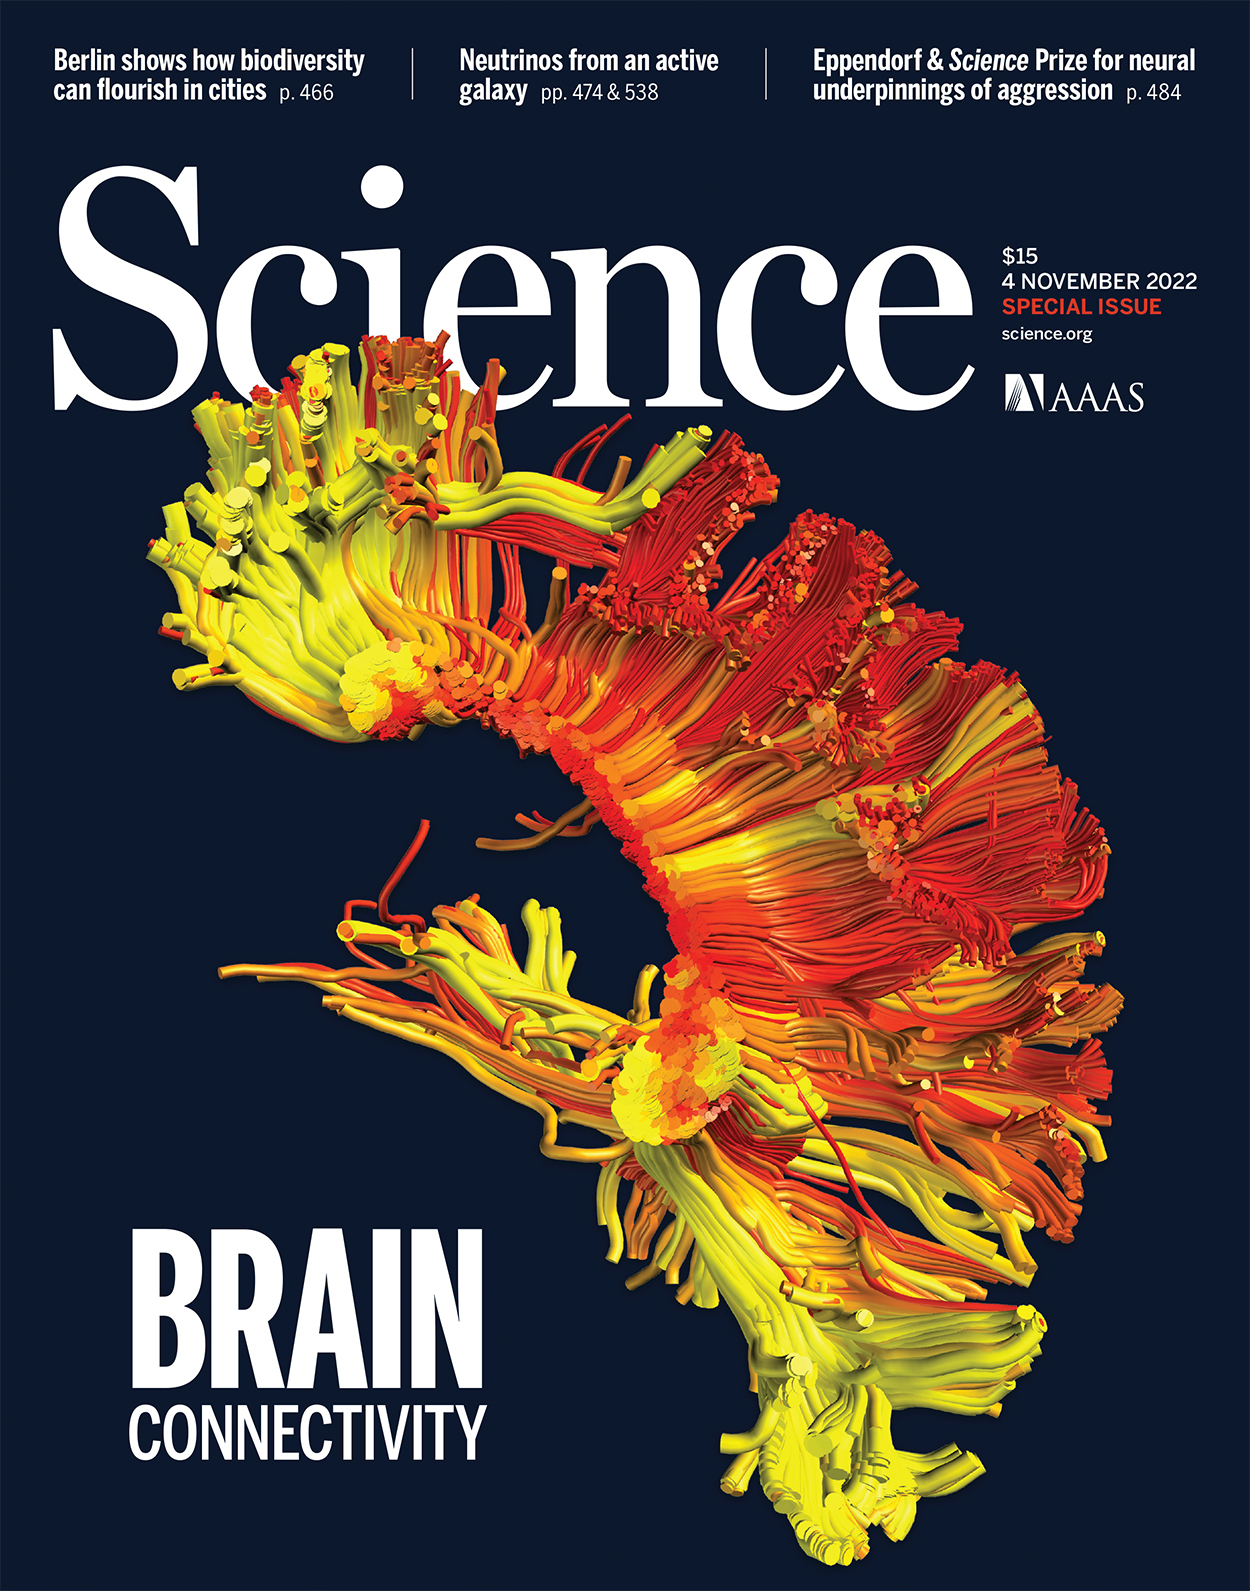
\includegraphics[width=0.3\linewidth]{imgs/connectome.jpg}
    \caption{Connectome}
    \label{fig:Connectome}
    \end{figure}
  
  \begin{itemize}
    \item Connectome是一个新兴的神经科学领域,它使用先进的神经成像和计算技术来
    构建和分析神经元之间的连接图谱
    \item VISoR是一个高通量高分辨率的全脑成像方法,已经完成了猴脑的全脑成像,并有望用于人脑
  \end{itemize}
\end{frame}

\begin{frame}[fragile]{任务}
  \begin{figure}[thbp!]
    \centering
    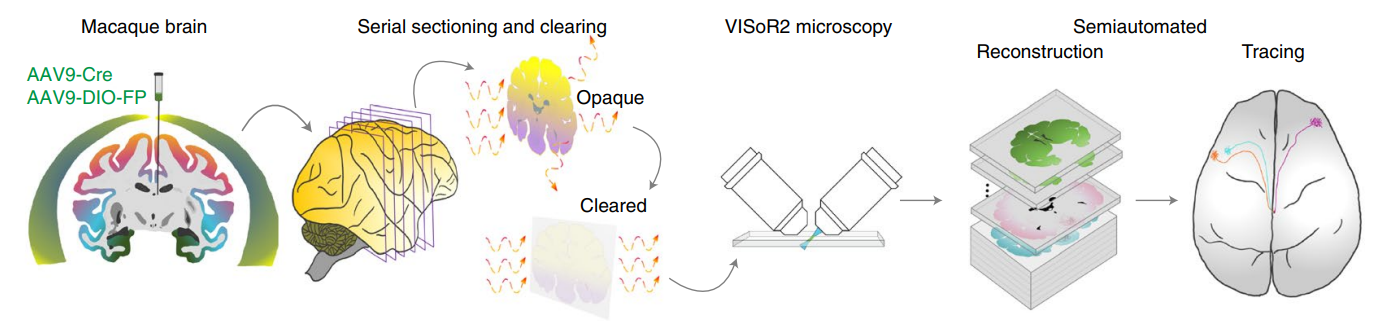
\includegraphics[width=1\linewidth]{imgs/VISoR.png}
    \caption{VISoR}
    \label{fig:VISoR}
    \end{figure}

  % \begin{itemize}
  %   \item VISoR成像中,需要对样本进行切割之后再成像,然后成的像需要拼接,拼接之后就可以进行神经元追踪,了解神经元之间的连接方式。
  %   \item 图像拼接是一个传统的计算机视觉的问题,主要应用场景的全景图像拼接,难点是大的视差。一般使用基于特征点匹配的全局单应性矩阵估计的算法。这类算法要求拼接的图像有较大的重叠区域。
  %   \item VISoR成像进行了样本切割后再成像,成的像之间无重叠区域,几乎所有的传统图像拼接算法全部失效。
  % \end{itemize}

  % 总的来说,就是要解决一个\textbf{无重叠区域的图像拼接问题}。

  \begin{itemize}
    \item 应用场景:VISoR\cite{xuHighthroughputMappingWhole2021}成像中样本切割成像后的图像拼接
    \item 难点:拼接的图像\textbf{无重叠区域}
    \item 相关工作:传统的图像拼接算法基本是基于\textbf{重叠区域特征匹配}和\textbf{单应性矩阵估计}的算法,要求拼接的图像间有较大的重叠区域
  \end{itemize}
\end{frame}

\section{方法}

\begin{frame}[fragile]{总览}
  \begin{enumerate}
    \item 使用加了平滑操作的基于DDPM\cite{ho2020denoising}的RePaint\cite{lugmayr2022repaint}对图像进行外插,修复出重叠区域
    \item 使用不同的相似度度量的标准找到生成区域中可能的重叠区域,然后拼接
  \end{enumerate}
\end{frame}

\begin{frame}[fragile]{DDPM}
  \begin{figure}[thbp!]
    \centering
    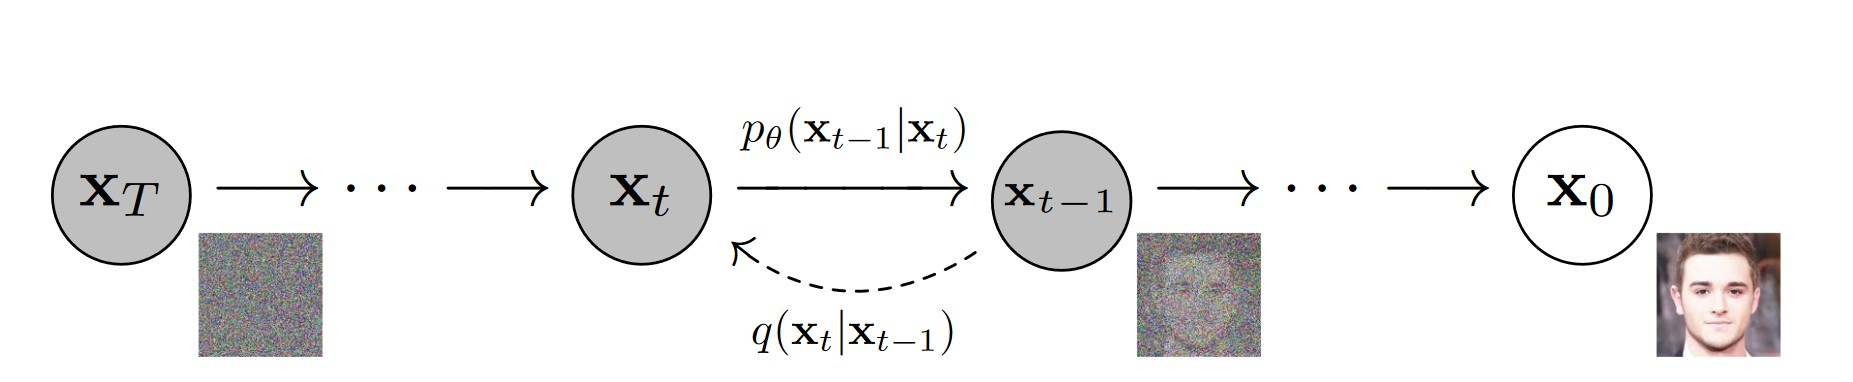
\includegraphics[width=1\linewidth]{imgs/DDPM.jpg}
    \caption{DDPM}
    \label{fig:DDPM}
    \end{figure}

  \begin{itemize}
    \item DDPM\cite{ho2020denoising}:Denoising Diffusion Probabilistic Models,是最近很火的AIGC的基础
    \item 将生成模型建模为加噪和去噪的两个马尔可夫随机过程
    \item 涉及的神经网络是用来估计噪声的加了positional encoding的U-Net
    \item 优化目标是$\theta = \operatorname{argmin}_{\theta} \mathbb{E}_{x_0,\epsilon}\left[\left\|\epsilon-\epsilon_\theta(\sqrt{\bar{\alpha}_t}x_0+\sqrt{1-\bar{\alpha}_t}\epsilon,t)\right\|^2\right] $
  \end{itemize}
\end{frame}

\begin{frame}[fragile]{RePaint}
  \begin{figure}[thbp!]
    \centering
    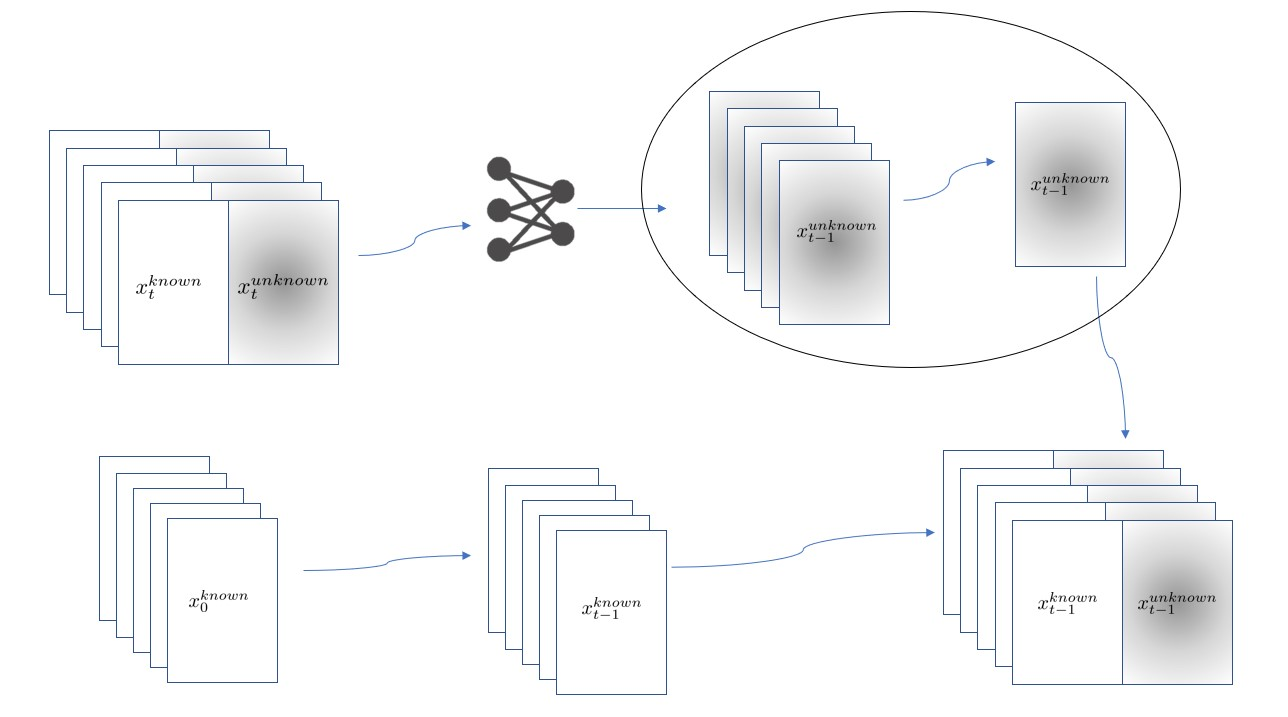
\includegraphics[width=0.6\linewidth]{imgs/RePaint.jpg}
    \caption{加了平滑操作的RePaint}
    \label{fig:RePaint}
    \end{figure}
  
  \begin{itemize}
    \item 图像修复是图像逆问题中的一种,图像逆问题可以建模为$y = Ax + \epsilon$
    \item RePaint\cite{lugmayr2022repaint}是一个基于DDPM的图像修复模型
    \item 通过反向过程中保留区域和要修复区域的线性组合来进行图像修复,通过resample的方法提高修复质量
    \item 我们给他加了一个平滑操作来进一步提升生成效果
  \end{itemize}

\end{frame}

\begin{frame}[fragile]{图像拼接}
  \begin{figure}[thbp!]
    \centering
    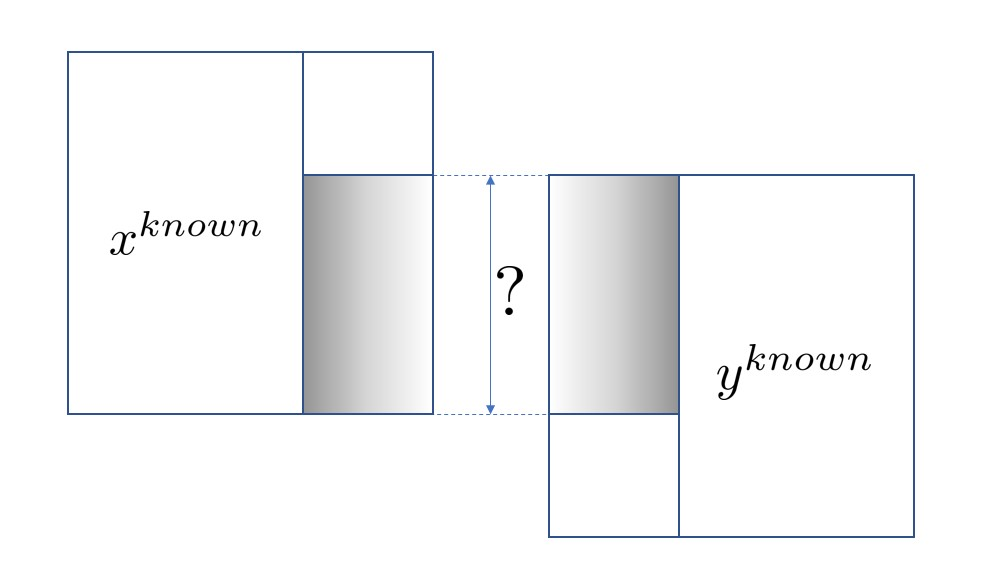
\includegraphics[width=0.6\linewidth]{imgs/stitch.jpg}
    \caption{图像拼接}
    \label{fig:stitch}
    \end{figure}

  \begin{itemize}
    \item 在使用图像修复模型对要拼接图像的边缘进行外插后,需要找到生成区域中最相似的区域来对图像进行配准
    \item 使用合适的图像相似度衡量算法来寻找图像间的位移,可以建模为$s = \mathop{\arg\max}\limits_{s} f_s(x, y)$
    \item $f$可以为MSE,PSNR,SSIM,NCC,COSSIM等
  \end{itemize}
\end{frame}

\section{结果}

\begin{frame}[fragile]{无条件生成}
  \begin{figure}[htbp]
    \centering
    \begin{minipage}[t]{0.49\textwidth}
    \centering
    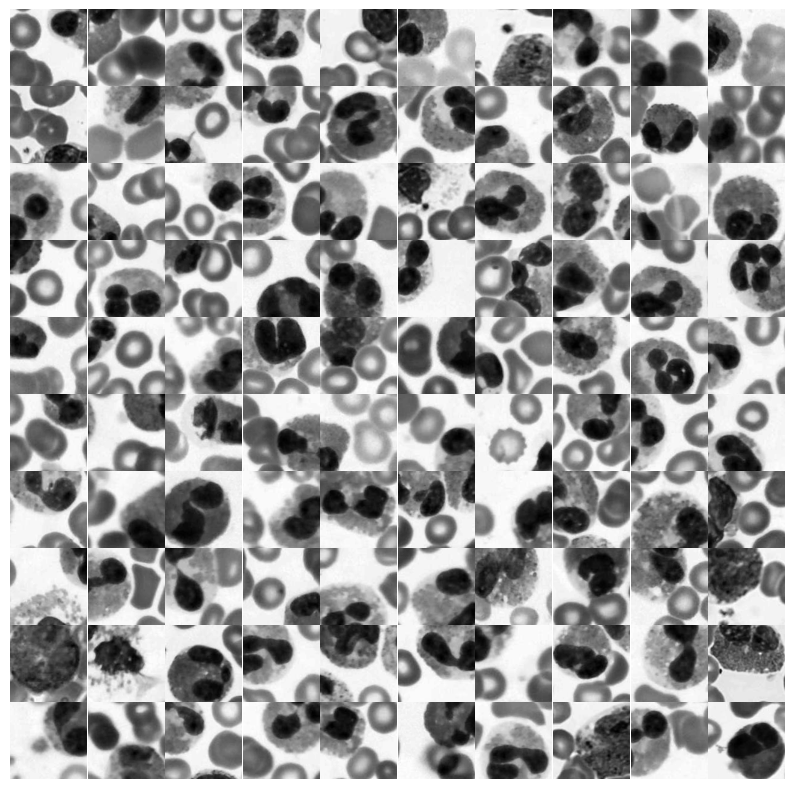
\includegraphics[width=1\linewidth]{imgs/gt.png}
    \caption{ground truth}
    \label{fig:gt}
    \end{minipage}
    \begin{minipage}[t]{0.49\textwidth}
    \centering
    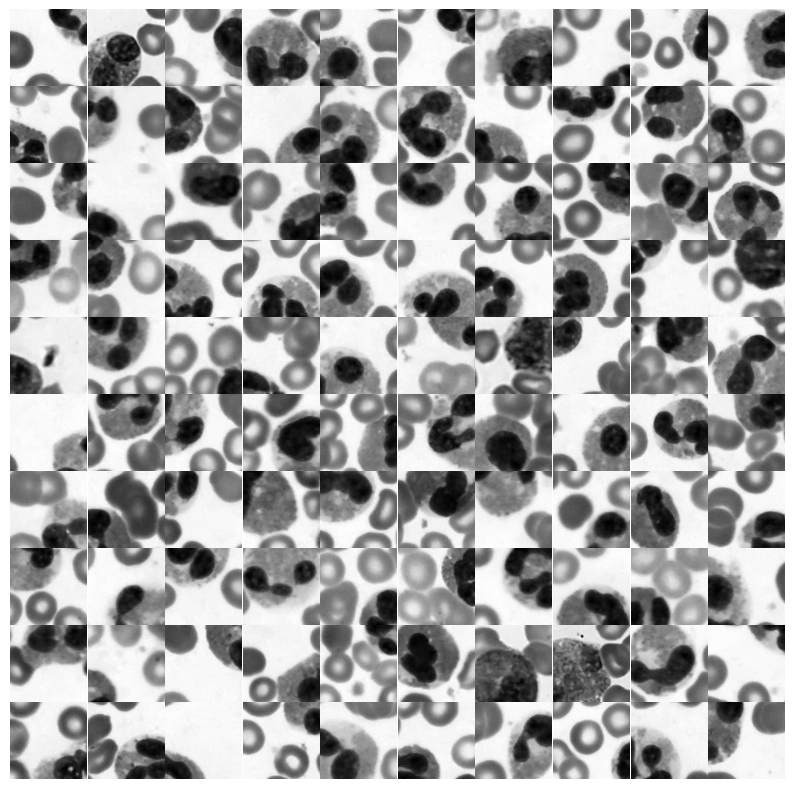
\includegraphics[width=1\linewidth]{imgs/uncon.png}
    \caption{无条件生成}
    \label{fig:uncon}
    \end{minipage}
    \end{figure}

  用来测试的是白细胞数据集\cite{kouzehkananLargeDatasetWhite2022},可以在kaggle下载。
  在原数据集和DDPM中随机采样了$10 \times 10$张图片,分别如图\ref{fig:gt}和图\ref{fig:uncon}所示。
\end{frame}

\begin{frame}[fragile]{图像修复}
  \begin{figure}[htbp]
    \centering
    \begin{minipage}[t]{0.49\textwidth}
    \centering
    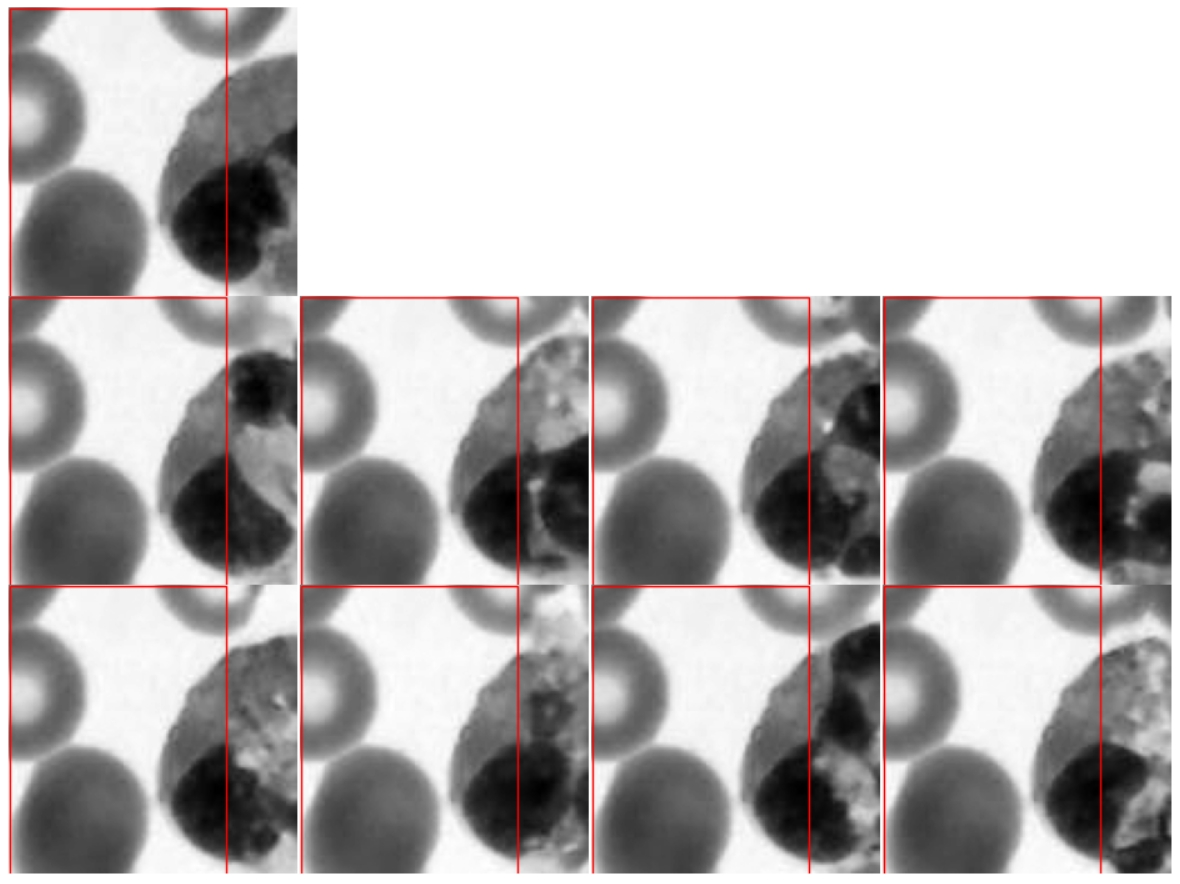
\includegraphics[width=1\linewidth]{imgs/con_unsmooth.jpg}
    \caption{RePaint}
    \label{fig:con_unsmooth}
    \end{minipage}
    \begin{minipage}[t]{0.49\textwidth}
    \centering
    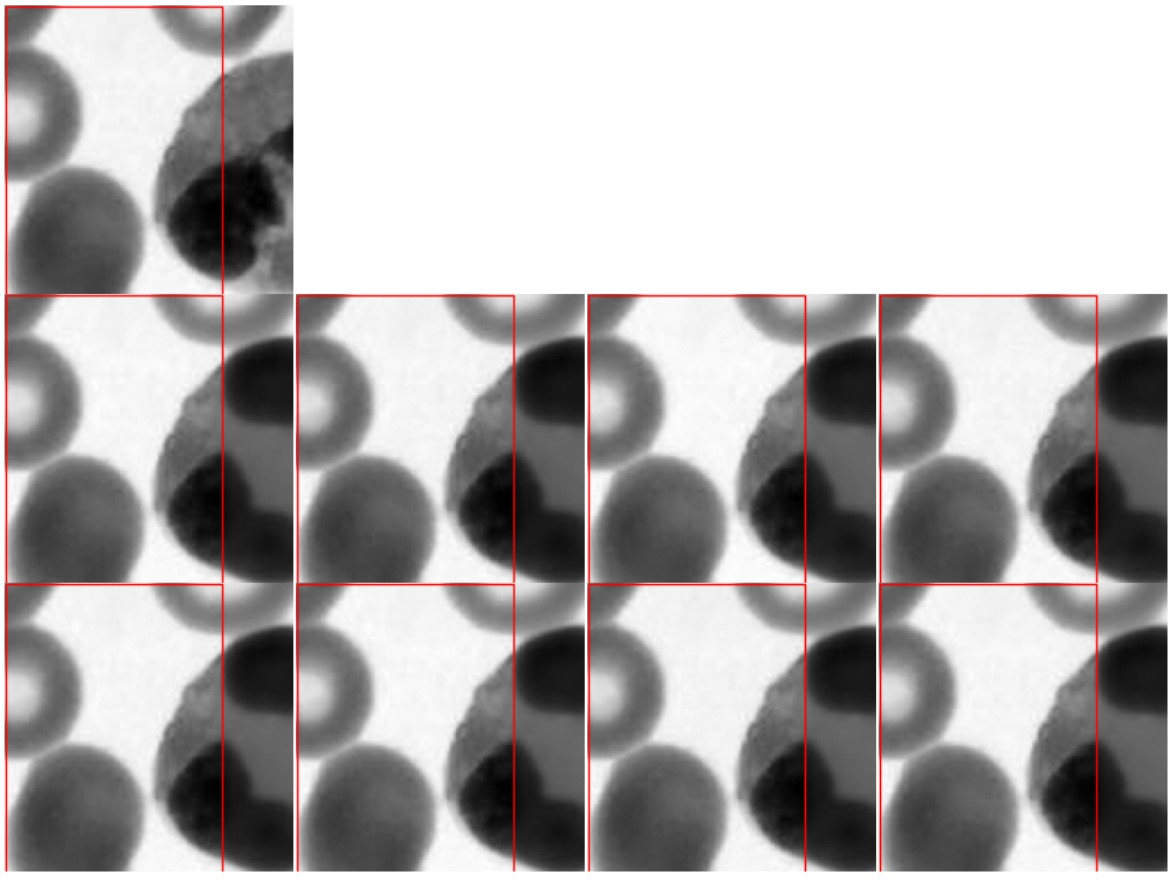
\includegraphics[width=1\linewidth]{imgs/con_smooth.jpg}
    \caption{加了平滑操作的RePaint}
    \label{fig:con_smooth}
    \end{minipage}
    \end{figure}

  原始的RePaint和加了平滑操作的RePaint对图片外插的结果,分别如图\ref{fig:con_unsmooth}和图\ref{fig:con_smooth}所示。
\end{frame}

\begin{frame}[fragile]{图像拼接}
  \begin{figure}[htbp]
    \centering
    \begin{minipage}[t]{0.49\textwidth}
    \centering
    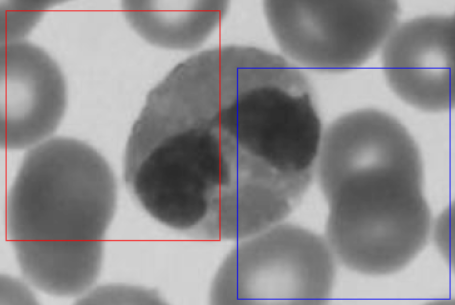
\includegraphics[width=1\linewidth]{imgs/gt_image.png}
    \caption{ground truth}
    \end{minipage}
    \begin{minipage}[t]{0.49\textwidth}
    \centering
    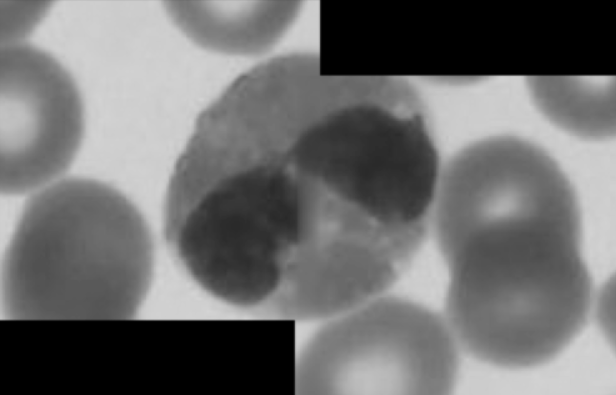
\includegraphics[width=1\linewidth]{imgs/result_image.png}
    \caption{图像拼接}
    \label{fig:res}
    \end{minipage}
    \end{figure}
  
  在测试了不同的$f$后,最终选择了SSIM,拼接的结果如图\ref{fig:res}所示。
\end{frame}

\section{展望}

\begin{frame}[fragile]{展望}
  \begin{itemize}
    \item 进一步提升拼接质量
    \item 2D -> 3D
    \item 使用真实的神经元数据集
    \item 生物图像 -> 自然图像
    \item 支持更多的图像变换
  \end{itemize}
\end{frame}

\begin{frame}[fragile]{致谢}
  \begin{itemize}
    \item 感谢陈亚雄老师的指导
    \item 感谢中科院深圳先进技术研究院周鹏程老师的指导和提高的计算设备
    \item 感谢DAMI-lab各位学长学姐的帮助
    \item 感谢父母和母校的培养
  \end{itemize}
\end{frame}

\appendix

\metroset{sectionpage=none}
\begin{frame}[allowframebreaks, noframenumbering]{References}
  \bibliography{demo}
  \bibliographystyle{unsrt}

\end{frame}


% \section{Introduction}

% \begin{frame}[fragile]{Metropolis}

%   The \themename theme is a Beamer theme with minimal visual noise
%   inspired by the \href{https://github.com/hsrmbeamertheme/hsrmbeamertheme}{\textsc{hsrm} Beamer
%   Theme} by Benjamin Weiss.

%   Enable the theme by loading

%   \begin{verbatim}    \documentclass{beamer}
%     \usetheme{metropolis}\end{verbatim}

%   Note, that you have to have Mozilla's \emph{Fira Sans} font and XeTeX
%   installed to enjoy this wonderful typography.
% \end{frame}
% \begin{frame}[fragile]{Sections}
%   Sections group slides of the same topic

%   \begin{verbatim}    \section{Elements}\end{verbatim}

%   for which \themename provides a nice progress indicator \ldots
% \end{frame}

% \section{Title formats}

% \begin{frame}{Metropolis title formats}
% 	\themename supports 4 different title formats:
% 	\begin{itemize}
% 		\item Regular
% 		\item \textsc{Small caps}
% 		\item \textsc{all small caps}
% 		\item ALL CAPS
% 	\end{itemize}
% 	They can either be set at once for every title type or individually.
% \end{frame}

% {
%     \metroset{titleformat frame=smallcaps}
% \begin{frame}{Small caps}
% 	This frame uses the \texttt{smallcaps} title format.

% 	\begin{alertblock}{Potential Problems}
% 		Be aware that not every font supports small caps. If for example you typeset your presentation with pdfTeX and the Computer Modern Sans Serif font, every text in small caps will be typeset with the Computer Modern Serif font instead.
% 	\end{alertblock}
% \end{frame}
% }

% {
% \metroset{titleformat frame=allsmallcaps}
% \begin{frame}{All small caps}
% 	This frame uses the \texttt{allsmallcaps} title format.

% 	\begin{alertblock}{Potential problems}
% 		As this title format also uses small caps you face the same problems as with the \texttt{smallcaps} title format. Additionally this format can cause some other problems. Please refer to the documentation if you consider using it.

% 		As a rule of thumb: just use it for plaintext-only titles.
% 	\end{alertblock}
% \end{frame}
% }

% {
% \metroset{titleformat frame=allcaps}
% \begin{frame}{All caps}
% 	This frame uses the \texttt{allcaps} title format.

% 	\begin{alertblock}{Potential Problems}
% 		This title format is not as problematic as the \texttt{allsmallcaps} format, but basically suffers from the same deficiencies. So please have a look at the documentation if you want to use it.
% 	\end{alertblock}
% \end{frame}
% }

% \section{Elements}

% \begin{frame}[fragile]{Typography}
%       \begin{verbatim}The theme provides sensible defaults to
% \emph{emphasize} text, \alert{accent} parts
% or show \textbf{bold} results.\end{verbatim}

%   \begin{center}becomes\end{center}

%   The theme provides sensible defaults to \emph{emphasize} text,
%   \alert{accent} parts or show \textbf{bold} results.
% \end{frame}

% \begin{frame}{Font feature test}
%   \begin{itemize}
%     \item Regular
%     \item \textit{Italic}
%     \item \textsc{Small Caps}
%     \item \textbf{Bold}
%     \item \textbf{\textit{Bold Italic}}
%     \item \textbf{\textsc{Bold Small Caps}}
%     \item \texttt{Monospace}
%     \item \texttt{\textit{Monospace Italic}}
%     \item \texttt{\textbf{Monospace Bold}}
%     \item \texttt{\textbf{\textit{Monospace Bold Italic}}}
%   \end{itemize}
% \end{frame}

% \begin{frame}{Lists}
%   \begin{columns}[T,onlytextwidth]
%     \column{0.33\textwidth}
%       Items
%       \begin{itemize}
%         \item Milk \item Eggs \item Potatoes
%       \end{itemize}

%     \column{0.33\textwidth}
%       Enumerations
%       \begin{enumerate}
%         \item First, \item Second and \item Last.
%       \end{enumerate}

%     \column{0.33\textwidth}
%       Descriptions
%       \begin{description}
%         \item[PowerPoint] Meeh. \item[Beamer] Yeeeha.
%       \end{description}
%   \end{columns}
% \end{frame}
% \begin{frame}{Animation}
%   \begin{itemize}[<+- | alert@+>]
%     \item \alert<4>{This is\only<4>{ really} important}
%     \item Now this
%     \item And now this
%   \end{itemize}
% \end{frame}
% \begin{frame}{Figures}
%   \begin{figure}
%     \newcounter{density}
%     \setcounter{density}{20}
%     \begin{tikzpicture}
%       \def\couleur{alerted text.fg}
%       \path[coordinate] (0,0)  coordinate(A)
%                   ++( 90:5cm) coordinate(B)
%                   ++(0:5cm) coordinate(C)
%                   ++(-90:5cm) coordinate(D);
%       \draw[fill=\couleur!\thedensity] (A) -- (B) -- (C) --(D) -- cycle;
%       \foreach \x in {1,...,40}{%
%           \pgfmathsetcounter{density}{\thedensity+20}
%           \setcounter{density}{\thedensity}
%           \path[coordinate] coordinate(X) at (A){};
%           \path[coordinate] (A) -- (B) coordinate[pos=.10](A)
%                               -- (C) coordinate[pos=.10](B)
%                               -- (D) coordinate[pos=.10](C)
%                               -- (X) coordinate[pos=.10](D);
%           \draw[fill=\couleur!\thedensity] (A)--(B)--(C)-- (D) -- cycle;
%       }
%     \end{tikzpicture}
%     \caption{Rotated square from
%     \href{http://www.texample.net/tikz/examples/rotated-polygons/}{texample.net}.}
%   \end{figure}
% \end{frame}
% \begin{frame}{Tables}
%   \begin{table}
%     \caption{Largest cities in the world (source: Wikipedia)}
%     \begin{tabular}{@{} lr @{}}
%       \toprule
%       City & Population\\
%       \midrule
%       Mexico City & 20,116,842\\
%       Shanghai & 19,210,000\\
%       Peking & 15,796,450\\
%       Istanbul & 14,160,467\\
%       \bottomrule
%     \end{tabular}
%   \end{table}
% \end{frame}
% \begin{frame}{Blocks}
%   Three different block environments are pre-defined and may be styled with an
%   optional background color.

%   \begin{columns}[T,onlytextwidth]
%     \column{0.5\textwidth}
%       \begin{block}{Default}
%         Block content.
%       \end{block}

%       \begin{alertblock}{Alert}
%         Block content.
%       \end{alertblock}

%       \begin{exampleblock}{Example}
%         Block content.
%       \end{exampleblock}

%     \column{0.5\textwidth}

%       \metroset{block=fill}

%       \begin{block}{Default}
%         Block content.
%       \end{block}

%       \begin{alertblock}{Alert}
%         Block content.
%       \end{alertblock}

%       \begin{exampleblock}{Example}
%         Block content.
%       \end{exampleblock}

%   \end{columns}
% \end{frame}
% \begin{frame}{Math}
%   \begin{equation*}
%     e = \lim_{n\to \infty} \left(1 + \frac{1}{n}\right)^n
%   \end{equation*}
% \end{frame}
% \begin{frame}{Line plots}
%   \begin{figure}
%     \begin{tikzpicture}
%       \begin{axis}[
%         mlineplot,
%         width=0.9\textwidth,
%         height=6cm,
%       ]

%         \addplot {sin(deg(x))};
%         \addplot+[samples=100] {sin(deg(2*x))};

%       \end{axis}
%     \end{tikzpicture}
%   \end{figure}
% \end{frame}
% \begin{frame}{Bar charts}
%   \begin{figure}
%     \begin{tikzpicture}
%       \begin{axis}[
%         mbarplot,
%         xlabel={Foo},
%         ylabel={Bar},
%         width=0.9\textwidth,
%         height=6cm,
%       ]

%       \addplot plot coordinates {(1, 20) (2, 25) (3, 22.4) (4, 12.4)};
%       \addplot plot coordinates {(1, 18) (2, 24) (3, 23.5) (4, 13.2)};
%       \addplot plot coordinates {(1, 10) (2, 19) (3, 25) (4, 15.2)};

%       \legend{lorem, ipsum, dolor}

%       \end{axis}
%     \end{tikzpicture}
%   \end{figure}
% \end{frame}
% \begin{frame}{Quotes}
%   \begin{quote}
%     Veni, Vidi, Vici
%   \end{quote}
% \end{frame}

% {%
% \setbeamertemplate{frame footer}{My custom footer}
% \begin{frame}[fragile]{Frame footer}
%     \themename defines a custom beamer template to add a text to the footer. It can be set via
%     \begin{verbatim}\setbeamertemplate{frame footer}{My custom footer}\end{verbatim}
% \end{frame}
% }

% \begin{frame}{References}
%   Some references to showcase [allowframebreaks] \cite{knuth92,ConcreteMath,Simpson,Er01,greenwade93}
% \end{frame}

% \section{Conclusion}

% \begin{frame}{Summary}

%   Get the source of this theme and the demo presentation from

%   \begin{center}\url{github.com/matze/mtheme}\end{center}

%   The theme \emph{itself} is licensed under a
%   \href{http://creativecommons.org/licenses/by-sa/4.0/}{Creative Commons
%   Attribution-ShareAlike 4.0 International License}.

%   \begin{center}\ccbysa\end{center}

% \end{frame}

% \begin{frame}[standout]
%   Questions?
% \end{frame}

% \appendix

% \begin{frame}[fragile]{Backup slides}
%   Sometimes, it is useful to add slides at the end of your presentation to
%   refer to during audience questions.

%   The best way to do this is to include the \verb|appendixnumberbeamer|
%   package in your preamble and call \verb|\appendix| before your backup slides.

%   \themename will automatically turn off slide numbering and progress bars for
%   slides in the appendix.
% \end{frame}

% \begin{frame}[allowframebreaks]{References}

%   \bibliography{demo}
%   \bibliographystyle{abbrv}

% \end{frame}

\begin{frame}[standout]
  THANKS
\end{frame}

\end{document}
